\documentclass[11pt,compress,t,notes=noshow, aspectratio=169, xcolor=table]{beamer}

\usepackage{../../style/lmu-lecture}
% Defines macros and environments
\usepackage[]{graphicx}
\usepackage[]{color}
% maxwidth is the original width if it is less than linewidth
% otherwise use linewidth (to make sure the graphics do not exceed the margin)
\makeatletter
\def\maxwidth{ %
\ifdim\Gin@nat@width>\linewidth
\linewidth
\else
\Gin@nat@width
\fi
}
\makeatother
%\usepackage[fontsize=10.5pt]{scrextend}
\definecolor{ggred}{rgb}{0.973, 0.463, 0.427}
\definecolor{ggblue}{rgb}{0, 0.749, 0.769}
\definecolor{fgcolor}{rgb}{0.345, 0.345, 0.345}
\newcommand{\hlnum}[1]{\textcolor[rgb]{0.686,0.059,0.569}{#1}}%
\newcommand{\hlstr}[1]{\textcolor[rgb]{0.192,0.494,0.8}{#1}}%
\newcommand{\hlcom}[1]{\textcolor[rgb]{0.678,0.584,0.686}{\textit{#1}}}%
\newcommand{\hlopt}[1]{\textcolor[rgb]{0,0,0}{#1}}%
\newcommand{\hlstd}[1]{\textcolor[rgb]{0.345,0.345,0.345}{#1}}%
\newcommand{\hlkwa}[1]{\textcolor[rgb]{0.161,0.373,0.58}{\textbf{#1}}}%
\newcommand{\hlkwb}[1]{\textcolor[rgb]{0.69,0.353,0.396}{#1}}%
\newcommand{\hlkwc}[1]{\textcolor[rgb]{0.333,0.667,0.333}{#1}}%
\newcommand{\hlkwd}[1]{\textcolor[rgb]{0.737,0.353,0.396}{\textbf{#1}}}%
\newcommand{\predvar}{Var\left[\hat{f}(\xv)\right]}
\let\hlipl\hlkwb

\usepackage{pdfpages}
\usepackage{framed}
\makeatletter
\newenvironment{kframe}{%
\def\at@end@of@kframe{}%
\ifinner\ifhmode%
\def\at@end@of@kframe{\end{minipage}}%
\begin{minipage}{\columnwidth}%
\fi\fi%
\def\FrameCommand##1{\hskip\@totalleftmargin \hskip-\fboxsep
\colorbox{shadecolor}{##1}\hskip-\fboxsep
% There is no \\@totalrightmargin, so:
\hskip-\linewidth \hskip-\@totalleftmargin \hskip\columnwidth}%
\MakeFramed {\advance\hsize-\width
\@totalleftmargin\z@ \linewidth\hsize
\@setminipage}}%
{\par\unskip\endMakeFramed%
\at@end@of@kframe}
\makeatother

\definecolor{shadecolor}{rgb}{.97, .97, .97}
\definecolor{messagecolor}{rgb}{0, 0, 0}
\definecolor{warningcolor}{rgb}{1, 0, 1}
\definecolor{errorcolor}{rgb}{1, 0, 0}
\newenvironment{knitrout}{}{} % an empty environment to be redefined in TeX

\usepackage{alltt}
\newcommand{\SweaveOpts}[1]{}  % do not interfere with LaTeX
\newcommand{\SweaveInput}[1]{} % because they are not real TeX commands
\newcommand{\Sexpr}[1]{}       % will only be parsed by R

\usepackage[english]{babel}
\usepackage[utf8]{inputenc}

\usepackage[export]{adjustbox}
\usepackage{dsfont}
\usepackage{verbatim}
\usepackage{amsmath}
\usepackage{amsfonts}
\usepackage{bm}
\usepackage{csquotes}
\usepackage{multirow}
\usepackage{longtable}
\usepackage{booktabs}
\usepackage{enumerate}
\usepackage[absolute,overlay]{textpos}
\usepackage{psfrag}
\usepackage{algorithm}
\usepackage{algpseudocode}
\usepackage{eqnarray}
\usepackage{arydshln}
\usepackage{tabularx}
\usepackage{placeins}
\usepackage{tikz}
\usepackage{setspace}
\usepackage{colortbl}
\usepackage{mathtools}
\usepackage{wrapfig}
\usepackage{bm}
\usepackage[backend=biber]{biblatex}

\usetikzlibrary{tikzmark, shapes,arrows,automata,positioning,calc,chains,trees,  shadows, decorations.pathreplacing}
\tikzset{
%Define standard arrow tip
>=stealth',
%Define style for boxes
punkt/.style={
rectangle,
rounded corners,
draw=black, very thick,
text width=6.5em,
minimum height=2em,
text centered},
% Define arrow style
pil/.style={
->,
thick,
shorten <=2pt,
shorten >=2pt,}
}

\usepackage{subfig}

\usepackage{bbm}
%\newcommand\hmmax{0}
%\newcommand\bmmax{0}
% basic latex stuff
\newcommand{\pkg}[1]{{\fontseries{b}\selectfont #1}} %fontstyle for R packages
\newcommand{\lz}{\vspace{0.5cm}} %vertical space
\newcommand{\dlz}{\vspace{1cm}} %double vertical space
\newcommand{\oneliner}[1] % Oneliner for important statements
{\begin{block}{}\begin{center}\begin{Large}#1\end{Large}\end{center}\end{block}}

% Latexmath Notation
% math spaces
\ifdefined\N                                                                
\renewcommand{\N}{\mathds{N}} % N, naturals
\else \newcommand{\N}{\mathds{N}} \fi 
\newcommand{\Z}{\mathds{Z}} % Z, integers
\newcommand{\Q}{\mathds{Q}} % Q, rationals
\newcommand{\R}{\mathds{R}} % R, reals
\ifdefined\C 
  \renewcommand{\C}{\mathds{C}} % C, complex
\else \newcommand{\C}{\mathds{C}} \fi
\newcommand{\continuous}{\mathcal{C}} % C, space of continuous functions
\newcommand{\M}{\mathcal{M}} % machine numbers
\newcommand{\epsm}{\epsilon_m} % maximum error

% counting / finite sets
\newcommand{\setzo}{\{0, 1\}} % set 0, 1
\newcommand{\setmp}{\{-1, +1\}} % set -1, 1
\newcommand{\unitint}{[0, 1]} % unit interval

% basic math stuff
\newcommand{\xt}{\tilde x} % x tilde
\newcommand{\argmax}{\operatorname{arg\,max}} % argmax
\newcommand{\argmin}{\operatorname{arg\,min}} % argmin
\newcommand{\argminlim}{\mathop{\mathrm{arg\,min}}\limits} % argmax with limits
\newcommand{\argmaxlim}{\mathop{\mathrm{arg\,max}}\limits} % argmin with limits  
\newcommand{\sign}{\operatorname{sign}} % sign, signum
\newcommand{\I}{\mathbb{I}} % I, indicator
\newcommand{\order}{\mathcal{O}} % O, order
\newcommand{\pd}[2]{\frac{\partial{#1}}{\partial #2}} % partial derivative
\newcommand{\floorlr}[1]{\left\lfloor #1 \right\rfloor} % floor
\newcommand{\ceillr}[1]{\left\lceil #1 \right\rceil} % ceiling

% sums and products
\newcommand{\sumin}{\sum\limits_{i=1}^n} % summation from i=1 to n
\newcommand{\sumim}{\sum\limits_{i=1}^m} % summation from i=1 to m
\newcommand{\sumjn}{\sum\limits_{j=1}^n} % summation from j=1 to p
\newcommand{\sumjp}{\sum\limits_{j=1}^p} % summation from j=1 to p
\newcommand{\sumik}{\sum\limits_{i=1}^k} % summation from i=1 to k
\newcommand{\sumkg}{\sum\limits_{k=1}^g} % summation from k=1 to g
\newcommand{\sumjg}{\sum\limits_{j=1}^g} % summation from j=1 to g
\newcommand{\meanin}{\frac{1}{n} \sum\limits_{i=1}^n} % mean from i=1 to n
\newcommand{\meanim}{\frac{1}{m} \sum\limits_{i=1}^m} % mean from i=1 to n
\newcommand{\meankg}{\frac{1}{g} \sum\limits_{k=1}^g} % mean from k=1 to g
\newcommand{\prodin}{\prod\limits_{i=1}^n} % product from i=1 to n
\newcommand{\prodkg}{\prod\limits_{k=1}^g} % product from k=1 to g
\newcommand{\prodjp}{\prod\limits_{j=1}^p} % product from j=1 to p

% linear algebra
\newcommand{\one}{\boldsymbol{1}} % 1, unitvector
\newcommand{\zero}{\mathbf{0}} % 0-vector
\newcommand{\id}{\boldsymbol{I}} % I, identity
\newcommand{\diag}{\operatorname{diag}} % diag, diagonal
\newcommand{\trace}{\operatorname{tr}} % tr, trace
\newcommand{\spn}{\operatorname{span}} % span
\newcommand{\scp}[2]{\left\langle #1, #2 \right\rangle} % <.,.>, scalarproduct
\newcommand{\mat}[1]{\begin{pmatrix} #1 \end{pmatrix}} % short pmatrix command
\newcommand{\Amat}{\mathbf{A}} % matrix A
\newcommand{\Deltab}{\mathbf{\Delta}} % error term for vectors

% basic probability + stats
\renewcommand{\P}{\mathds{P}} % P, probability
\newcommand{\E}{\mathds{E}} % E, expectation
\newcommand{\var}{\mathsf{Var}} % Var, variance
\newcommand{\cov}{\mathsf{Cov}} % Cov, covariance
\newcommand{\corr}{\mathsf{Corr}} % Corr, correlation
\newcommand{\normal}{\mathcal{N}} % N of the normal distribution
\newcommand{\iid}{\overset{i.i.d}{\sim}} % dist with i.i.d superscript
\newcommand{\distas}[1]{\overset{#1}{\sim}} % ... is distributed as ...

% machine learning
\newcommand{\Xspace}{\mathcal{X}} % X, input space
\newcommand{\Yspace}{\mathcal{Y}} % Y, output space
\newcommand{\nset}{\{1, \ldots, n\}} % set from 1 to n
\newcommand{\pset}{\{1, \ldots, p\}} % set from 1 to p
\newcommand{\gset}{\{1, \ldots, g\}} % set from 1 to g
\newcommand{\Pxy}{\mathbb{P}_{xy}} % P_xy
\newcommand{\Exy}{\mathbb{E}_{xy}} % E_xy: Expectation over random variables xy
\newcommand{\xv}{\mathbf{x}} % vector x (bold)
\newcommand{\xtil}{\tilde{\mathbf{x}}} % vector x-tilde (bold)
\newcommand{\yv}{\mathbf{y}} % vector y (bold)
\newcommand{\xy}{(\xv, y)} % observation (x, y)
\newcommand{\xvec}{\left(x_1, \ldots, x_p\right)^\top} % (x1, ..., xp) 
\newcommand{\Xmat}{\mathbf{X}} % Design matrix
\newcommand{\allDatasets}{\mathds{D}} % The set of all datasets
\newcommand{\allDatasetsn}{\mathds{D}_n}  % The set of all datasets of size n 
\newcommand{\D}{\mathcal{D}} % D, data
\newcommand{\Dn}{\D_n} % D_n, data of size n
\newcommand{\Dtrain}{\mathcal{D}_{\text{train}}} % D_train, training set
\newcommand{\Dtest}{\mathcal{D}_{\text{test}}} % D_test, test set
\newcommand{\xyi}[1][i]{\left(\xv^{(#1)}, y^{(#1)}\right)} % (x^i, y^i), i-th observation
\newcommand{\Dset}{\left( \xyi[1], \ldots, \xyi[n]\right)} % {(x1,y1)), ..., (xn,yn)}, data
\newcommand{\defAllDatasetsn}{(\Xspace \times \Yspace)^n} % Def. of the set of all datasets of size n 
\newcommand{\defAllDatasets}{\bigcup_{n \in \N}(\Xspace \times \Yspace)^n} % Def. of the set of all datasets 
\newcommand{\xdat}{\left\{ \xv^{(1)}, \ldots, \xv^{(n)}\right\}} % {x1, ..., xn}, input data
\newcommand{\ydat}{\left\{ \yv^{(1)}, \ldots, \yv^{(n)}\right\}} % {y1, ..., yn}, input data
\newcommand{\yvec}{\left(y^{(1)}, \hdots, y^{(n)}\right)^\top} % (y1, ..., yn), vector of outcomes
\renewcommand{\xi}[1][i]{\xv^{(#1)}} % x^i, i-th observed value of x
\newcommand{\yi}[1][i]{y^{(#1)}} % y^i, i-th observed value of y 
\newcommand{\xivec}{\left(x^{(i)}_1, \ldots, x^{(i)}_p\right)^\top} % (x1^i, ..., xp^i), i-th observation vector
\newcommand{\xj}{\xv_j} % x_j, j-th feature
\newcommand{\xjvec}{\left(x^{(1)}_j, \ldots, x^{(n)}_j\right)^\top} % (x^1_j, ..., x^n_j), j-th feature vector
\newcommand{\phiv}{\mathbf{\phi}} % Basis transformation function phi
\newcommand{\phixi}{\mathbf{\phi}^{(i)}} % Basis transformation of xi: phi^i := phi(xi)

%%%%%% ml - models general
\newcommand{\lamv}{\bm{\lambda}} % lambda vector, hyperconfiguration vector
\newcommand{\Lam}{\bm{\Lambda}}	 % Lambda, space of all hpos
% Inducer / Inducing algorithm
\newcommand{\preimageInducer}{\left(\defAllDatasets\right)\times\Lam} % Set of all datasets times the hyperparameter space
\newcommand{\preimageInducerShort}{\allDatasets\times\Lam} % Set of all datasets times the hyperparameter space
% Inducer / Inducing algorithm
\newcommand{\ind}{\mathcal{I}} % Inducer, inducing algorithm, learning algorithm 

% continuous prediction function f
\newcommand{\ftrue}{f_{\text{true}}}  % True underlying function (if a statistical model is assumed)
\newcommand{\ftruex}{\ftrue(\xv)} % True underlying function (if a statistical model is assumed)
\newcommand{\fx}{f(\xv)} % f(x), continuous prediction function
\newcommand{\fdomains}{f: \Xspace \rightarrow \R^g} % f with domain and co-domain
\newcommand{\Hspace}{\mathcal{H}} % hypothesis space where f is from
\newcommand{\fbayes}{f^{\ast}} % Bayes-optimal model
\newcommand{\fxbayes}{f^{\ast}(\xv)} % Bayes-optimal model
\newcommand{\fkx}[1][k]{f_{#1}(\xv)} % f_j(x), discriminant component function
\newcommand{\fh}{\hat{f}} % f hat, estimated prediction function
\newcommand{\fxh}{\fh(\xv)} % fhat(x)
\newcommand{\fxt}{f(\xv ~|~ \thetab)} % f(x | theta)
\newcommand{\fxi}{f\left(\xv^{(i)}\right)} % f(x^(i))
\newcommand{\fxih}{\hat{f}\left(\xv^{(i)}\right)} % f(x^(i))
\newcommand{\fxit}{f\left(\xv^{(i)} ~|~ \thetab\right)} % f(x^(i) | theta)
\newcommand{\fhD}{\fh_{\D}} % fhat_D, estimate of f based on D
\newcommand{\fhDtrain}{\fh_{\Dtrain}} % fhat_Dtrain, estimate of f based on D
\newcommand{\fhDnlam}{\fh_{\Dn, \lamv}} %model learned on Dn with hp lambda
\newcommand{\fhDlam}{\fh_{\D, \lamv}} %model learned on D with hp lambda
\newcommand{\fhDnlams}{\fh_{\Dn, \lamv^\ast}} %model learned on Dn with optimal hp lambda 
\newcommand{\fhDlams}{\fh_{\D, \lamv^\ast}} %model learned on D with optimal hp lambda 

% discrete prediction function h
\newcommand{\hx}{h(\xv)} % h(x), discrete prediction function
\newcommand{\hh}{\hat{h}} % h hat
\newcommand{\hxh}{\hat{h}(\xv)} % hhat(x)
\newcommand{\hxt}{h(\xv | \thetab)} % h(x | theta)
\newcommand{\hxi}{h\left(\xi\right)} % h(x^(i))
\newcommand{\hxit}{h\left(\xi ~|~ \thetab\right)} % h(x^(i) | theta)
\newcommand{\hbayes}{h^{\ast}} % Bayes-optimal classification model
\newcommand{\hxbayes}{h^{\ast}(\xv)} % Bayes-optimal classification model

% yhat
\newcommand{\yh}{\hat{y}} % yhat for prediction of target
\newcommand{\yih}{\hat{y}^{(i)}} % yhat^(i) for prediction of ith targiet
\newcommand{\resi}{\yi- \yih}

% theta
\newcommand{\thetah}{\hat{\theta}} % theta hat
\newcommand{\thetab}{\bm{\theta}} % theta vector
\newcommand{\thetabh}{\bm{\hat\theta}} % theta vector hat
\newcommand{\thetat}[1][t]{\thetab^{[#1]}} % theta^[t] in optimization
\newcommand{\thetatn}[1][t]{\thetab^{[#1 +1]}} % theta^[t+1] in optimization
\newcommand{\thetahDnlam}{\thetabh_{\Dn, \lamv}} %theta learned on Dn with hp lambda
\newcommand{\thetahDlam}{\thetabh_{\D, \lamv}} %theta learned on D with hp lambda
\newcommand{\mint}{\min_{\thetab \in \Theta}} % min problem theta
\newcommand{\argmint}{\argmin_{\thetab \in \Theta}} % argmin theta

% densities + probabilities
% pdf of x 
\newcommand{\pdf}{p} % p
\newcommand{\pdfx}{p(\xv)} % p(x)
\newcommand{\pixt}{\pi(\xv~|~ \thetab)} % pi(x|theta), pdf of x given theta
\newcommand{\pixit}[1][i]{\pi\left(\xi[#1] ~|~ \thetab\right)} % pi(x^i|theta), pdf of x given theta
\newcommand{\pixii}[1][i]{\pi\left(\xi[#1]\right)} % pi(x^i), pdf of i-th x 

% pdf of (x, y)
\newcommand{\pdfxy}{p(\xv,y)} % p(x, y)
\newcommand{\pdfxyt}{p(\xv, y ~|~ \thetab)} % p(x, y | theta)
\newcommand{\pdfxyit}{p\left(\xi, \yi ~|~ \thetab\right)} % p(x^(i), y^(i) | theta)

% pdf of x given y
\newcommand{\pdfxyk}[1][k]{p(\xv | y= #1)} % p(x | y = k)
\newcommand{\lpdfxyk}[1][k]{\log p(\xv | y= #1)} % log p(x | y = k)
\newcommand{\pdfxiyk}[1][k]{p\left(\xi | y= #1 \right)} % p(x^i | y = k)

% prior probabilities
\newcommand{\pik}[1][k]{\pi_{#1}} % pi_k, prior
\newcommand{\lpik}[1][k]{\log \pi_{#1}} % log pi_k, log of the prior
\newcommand{\pit}{\pi(\thetab)} % Prior probability of parameter theta

% posterior probabilities
\newcommand{\post}{\P(y = 1 ~|~ \xv)} % P(y = 1 | x), post. prob for y=1
\newcommand{\postk}[1][k]{\P(y = #1 ~|~ \xv)} % P(y = k | y), post. prob for y=k
\newcommand{\pidomains}{\pi: \Xspace \rightarrow \unitint} % pi with domain and co-domain
\newcommand{\pibayes}{\pi^{\ast}} % Bayes-optimal classification model
\newcommand{\pixbayes}{\pi^{\ast}(\xv)} % Bayes-optimal classification model
\newcommand{\pix}{\pi(\xv)} % pi(x), P(y = 1 | x)
\newcommand{\piv}{\bm{\pi}} % pi, bold, as vector
\newcommand{\pikx}[1][k]{\pi_{#1}(\xv)} % pi_k(x), P(y = k | x)
\newcommand{\pikxt}[1][k]{\pi_{#1}(\xv ~|~ \thetab)} % pi_k(x | theta), P(y = k | x, theta)
\newcommand{\pixh}{\hat \pi(\xv)} % pi(x) hat, P(y = 1 | x) hat
\newcommand{\pikxh}[1][k]{\hat \pi_{#1}(\xv)} % pi_k(x) hat, P(y = k | x) hat
\newcommand{\pixih}{\hat \pi(\xi)} % pi(x^(i)) with hat
\newcommand{\pikxih}[1][k]{\hat \pi_{#1}(\xi)} % pi_k(x^(i)) with hat
\newcommand{\pdfygxt}{p(y ~|~\xv, \thetab)} % p(y | x, theta)
\newcommand{\pdfyigxit}{p\left(\yi ~|~\xi, \thetab\right)} % p(y^i |x^i, theta)
\newcommand{\lpdfygxt}{\log \pdfygxt } % log p(y | x, theta)
\newcommand{\lpdfyigxit}{\log \pdfyigxit} % log p(y^i |x^i, theta)

% probababilistic
\newcommand{\bayesrulek}[1][k]{\frac{\P(\xv | y= #1) \P(y= #1)}{\P(\xv)}} % Bayes rule
\newcommand{\muk}{\bm{\mu_k}} % mean vector of class-k Gaussian (discr analysis) 

% residual and margin
\newcommand{\eps}{\epsilon} % residual, stochastic
\newcommand{\epsi}{\epsilon^{(i)}} % epsilon^i, residual, stochastic
\newcommand{\epsh}{\hat{\epsilon}} % residual, estimated
\newcommand{\yf}{y \fx} % y f(x), margin
\newcommand{\yfi}{\yi \fxi} % y^i f(x^i), margin
\newcommand{\Sigmah}{\hat \Sigma} % estimated covariance matrix
\newcommand{\Sigmahj}{\hat \Sigma_j} % estimated covariance matrix for the j-th class

% ml - loss, risk, likelihood
\newcommand{\Lyf}{L\left(y, f\right)} % L(y, f), loss function
\newcommand{\Lypi}{L\left(y, \pi\right)} % L(y, pi), loss function
\newcommand{\Lxy}{L\left(y, \fx\right)} % L(y, f(x)), loss function
\newcommand{\Lxyi}{L\left(\yi, \fxi\right)} % loss of observation
\newcommand{\Lxyt}{L\left(y, \fxt\right)} % loss with f parameterized
\newcommand{\Lxyit}{L\left(\yi, \fxit\right)} % loss of observation with f parameterized
\newcommand{\Lxym}{L\left(\yi, f\left(\bm{\tilde{x}}^{(i)} ~|~ \thetab\right)\right)} % loss of observation with f parameterized
\newcommand{\Lpixy}{L\left(y, \pix\right)} % loss in classification
\newcommand{\Lpiv}{L\left(y, \piv\right)} % loss in classification
\newcommand{\Lpixyi}{L\left(\yi, \pixii\right)} % loss of observation in classification
\newcommand{\Lpixyt}{L\left(y, \pixt\right)} % loss with pi parameterized
\newcommand{\Lpixyit}{L\left(\yi, \pixit\right)} % loss of observation with pi parameterized
\newcommand{\Lhxy}{L\left(y, \hx\right)} % L(y, h(x)), loss function on discrete classes
\newcommand{\Lr}{L\left(r\right)} % L(r), loss defined on residual (reg) / margin (classif)
\newcommand{\lone}{|y - \fx|} % L1 loss
\newcommand{\ltwo}{\left(y - \fx\right)^2} % L2 loss
\newcommand{\lbernoullimp}{\ln(1 + \exp(-y \cdot \fx))} % Bernoulli loss for -1, +1 encoding
\newcommand{\lbernoullizo}{- y \cdot \fx + \log(1 + \exp(\fx))} % Bernoulli loss for 0, 1 encoding
\newcommand{\lcrossent}{- y \log \left(\pix\right) - (1 - y) \log \left(1 - \pix\right)} % cross-entropy loss
\newcommand{\lbrier}{\left(\pix - y \right)^2} % Brier score
\newcommand{\risk}{\mathcal{R}} % R, risk
\newcommand{\riskbayes}{\mathcal{R}^\ast}
\newcommand{\riskf}{\risk(f)} % R(f), risk
\newcommand{\riskdef}{\E_{y|\xv}\left(\Lxy \right)} % risk def (expected loss)
\newcommand{\riskt}{\mathcal{R}(\thetab)} % R(theta), risk
\newcommand{\riske}{\mathcal{R}_{\text{emp}}} % R_emp, empirical risk w/o factor 1 / n
\newcommand{\riskeb}{\bar{\mathcal{R}}_{\text{emp}}} % R_emp, empirical risk w/ factor 1 / n
\newcommand{\riskef}{\riske(f)} % R_emp(f)
\newcommand{\risket}{\mathcal{R}_{\text{emp}}(\thetab)} % R_emp(theta)
\newcommand{\riskr}{\mathcal{R}_{\text{reg}}} % R_reg, regularized risk
\newcommand{\riskrt}{\mathcal{R}_{\text{reg}}(\thetab)} % R_reg(theta)
\newcommand{\riskrf}{\riskr(f)} % R_reg(f)
\newcommand{\riskrth}{\hat{\mathcal{R}}_{\text{reg}}(\thetab)} % hat R_reg(theta)
\newcommand{\risketh}{\hat{\mathcal{R}}_{\text{emp}}(\thetab)} % hat R_emp(theta)
\newcommand{\LL}{\mathcal{L}} % L, likelihood
\newcommand{\LLt}{\mathcal{L}(\thetab)} % L(theta), likelihood
\newcommand{\LLtx}{\mathcal{L}(\thetab | \xv)} % L(theta|x), likelihood
\newcommand{\logl}{\ell} % l, log-likelihood
\newcommand{\loglt}{\logl(\thetab)} % l(theta), log-likelihood
\newcommand{\logltx}{\logl(\thetab | \xv)} % l(theta|x), log-likelihood
\newcommand{\errtrain}{\text{err}_{\text{train}}} % training error
\newcommand{\errtest}{\text{err}_{\text{test}}} % test error
\newcommand{\errexp}{\overline{\text{err}_{\text{test}}}} % avg training error

% lm
\newcommand{\thx}{\thetab^\top \xv} % linear model
\newcommand{\olsest}{(\Xmat^\top \Xmat)^{-1} \Xmat^\top \yv} % OLS estimator in LM 

%%%%%% perturbed data
\usepackage{xifthen}
\newcommand{\pert}[3]{\ifthenelse{\equal{#2}{}}{\tilde{#1}}{\ifthenelse{\equal{#3}{}}{\tilde{#1}^{#2}}{\tilde{#1}^{#2|#3}}}}	% command to express that for #1 the subset #2 was perturbed given subset #3

%%%%%% marginalized functions
\newcommand{\fj}{f_j} % marginal function f_j, depending on feature j
\newcommand{\fnj}{f_{-j}} % marginal function f_{-j}, depending on all features but j
\newcommand{\fS}{f_S} % marginal function f_S depending on feature set S
\newcommand{\fnj}{f_{-S}} % marginal function f_{-S}, depending on all features but features in S
\newcommand{\fC}{f_C} % marginal function f_C depending on feature set C
\newcommand{\fhj}{\fh_j} % marginal function fh_j, depending on feature j
\newcommand{\fhnj}{\fh_{-j}} % marginal function fh_{-j}, depending on all features but j
\newcommand{\fhS}{\fh_S} % marginal function fh_S depending on feature set S
\newcommand{\fhnS}{\fh_{-S}} % marginal function fh_{-S}, depending on all features but features in S
\newcommand{\fhC}{\fh_C} % marginal function fh_C depending on feature set C
\newcommand{\XSmat}{\Xmat_S} % Design matrix subset
\newcommand{\XnSmat}{\Xmat__{-S}} % Design matrix subset without S
\newcommand{\XCmat}{\Xmat_C} % Design matrix subset
\newcommand{\Xnj}{\Xmat_{-j}} % Design matrix subset -j = {1, .., j-1, j+1, ..., p}

%%%%% Shapley values
\newcommand{\Scupj}{S \cup \{j\}} % coalition S but without player j
\newcommand{\Scupk}{S \cup \{k\}} % coalition S but without player k
\newcommand{\SsubP}{S \subseteq P} % coalition S subset of P
\newcommand{\SsubPnoj}{\SsubP \setminus \{j\}} % coalition S subset of P without player j
\newcommand{\SsubPnojk}{\SsubP \setminus \{j,k\}} % coalition S subset of P without player k
\newcommand{\phiij}{\hat{\phi}_j^{(i)}} % Shapley value for feature j and observation i

%%%%% LIME 
\newcommand{\Gspace}{\mathcal{G}} % Hypothesis space for surrogate model
\newcommand{\neigh}{\phi_{\xv}} % Proximity measure
\newcommand{\zv}{\mathbf{z}} % Sampled datapoints for surrogate
\newcommand{\Zspace}{\mathcal{Z}} % Space of sampled datapoints
\newcommand{\Gower}{d_G} % Gower distance


\newcommand{\indep}{\perp}
\newcommand{\Ind}{\mathcal{I}}

%new environments
\newenvironment{vbframe}  %frame with breaks and verbatim
{
\begin{frame}%[containsverbatim,allowframebreaks]
}
{
\end{frame}
}

% \newenvironment{vframe}  %frame with verbatim without breaks (to avoid numbering one slided frames)
% {
%  \begin{frame}[containsverbatim]
% }
% {
% \end{frame}
% }

\newenvironment{blocki}[1]   % itemize block
{
 \begin{block}{#1}\begin{itemize}
}
{
\end{itemize}\end{block}
}

\newenvironment{fragileframe}[2]{  %fragile frame with framebreaks
\begin{frame}[allowframebreaks, fragile, environment = fragileframe]
\frametitle{#1}
#2}
{\end{frame}}


\newcommand{\myframe}[2]{  %short for frame with framebreaks
\begin{frame}[allowframebreaks]
\frametitle{#1}
#2
\end{frame}}

\newcommand{\remark}[1]{
  \textbf{Remark:} #1
}


\newenvironment{deleteframe}
{
\begingroup
\usebackgroundtemplate{
\includegraphics[width=\paperwidth,height=\paperheight]{../style/color/red.png}}
 \begin{frame}
}
{
\end{frame}
\endgroup
}
\newenvironment{simplifyframe}
{
\begingroup
\usebackgroundtemplate{
\includegraphics[width=\paperwidth,height=\paperheight]{../style/color/yellow.png}}
 \begin{frame}
}
{
\end{frame}
\endgroup
}\newenvironment{draftframe}
{
\begingroup
\usebackgroundtemplate{
\includegraphics[width=\paperwidth,height=\paperheight]{../style/color/green.jpg}}
 \begin{frame}
}
{
\end{frame}
\endgroup
}
% https://tex.stackexchange.com/a/261480: textcolor that works in mathmode
\makeatletter
\renewcommand*{\@textcolor}[3]{%
  \protect\leavevmode
  \begingroup
    \color#1{#2}#3%
  \endgroup
}
\makeatother

% \makeatletter
% %\newcommand\notsotiny{\@setfontsize\notsotiny\@vipt\@viipt}
% \newcommand\notsotiny{\@setfontsize\notsotiny{6.31415}{7.1828}}
% \makeatother

\providecommand{\tightlist}{%
  \setlength{\itemsep}{0pt}\setlength{\parskip}{0pt}}

%\setbeamerfont{footnote}{size=\tiny}
\usepackage[hang,flushmargin]{footmisc}
\renewcommand*{\footnotelayout}{\tiny}
\renewcommand*{\thefootnote}{} %\fnsymbol{footnote}

% https://tex.stackexchange.com/questions/638616/beamer-frametitle-always-uppercase-for-text-but-not-for-href-or-url
\usepackage{textcase}

% https://stackoverflow.com/questions/377301/is-there-a-latex-command-to-make-text-all-lower-caps
%\usepackage[overload]{textcase}
%\setbeamertemplate{frametitle}{\MakeTextUppercase{\insertframetitle}}
%\setbeamertemplate{frametitle}{\expandafter\uppercase\expandafter\insertframetitle}

\setbeamertemplate{frametitle}{\MakeTextUppercase{\insertframetitle}}
\newcommand{\citebutton}[2]{%
\NoCaseChange{\resizebox{!}{9pt}{\protect\beamergotobutton{\href{#2}{#1}}}}%
}

%\setbeamertemplate{frametitle}{\expandafter\uppercase\expandafter\insertframetitle}
%\newcommand{\citebutton}[2]{%
%\href{#2}{\footnotesize\color{black!60}[#1]}
%\resizebox{!}{9pt}{\beamergotobutton{\lowercase{\href{#2}}{#1}}}% \MakeLowercase
%}
%\newcommand{\lit}[2]{\href{#2}{\footnotesize\color{black!60}[#1]}}

\newcommand{\lit}[2]{\href{#2}{\footnotesize\color{black!60}[#1]}}

\let\code=\texttt
\let\proglang=\textsf

\setkeys{Gin}{width=0.9\textwidth}

% https://tex.stackexchange.com/questions/30720/footnote-without-a-marker
% \makeatletter
% \def\blfootnote{\gdef\@thefnmark{}\@footnotetext}
% \makeatother

% https://tex.stackexchange.com/questions/357717/beamer-allowframebreaks-option-and-vertical-spacing-when-using-lists-itemize
% \setbeamertemplate{frametitle continuation}{%
%     (\insertcontinuationcount)%
%     \ifnum\insertcontinuationcount>1%
%     \vspace*{\topsep}%
%     \else%
%     %
%     \fi%
% }


\title{Interpretable Machine Learning}
% \author{LMU}
%\institute{\href{https://compstat-lmu.github.io/lecture_iml/}{compstat-lmu.github.io/lecture\_iml}}
\date{}

\begin{document}

\newcommand{\titlefigure}{figure_man/bike-sharing03.png}
\newcommand{\learninggoals}{
\item See model predictions as a cooperative game
\item Transfer the Shapley value concept from game theory to machine learning
}

\lecturechapter{Shapley Values for Local Explanations}
\lecture{Interpretable Machine Learning}


\begin{vbframe}{From Game Theory To Machine Learning}

\begin{figure}
    \centering
    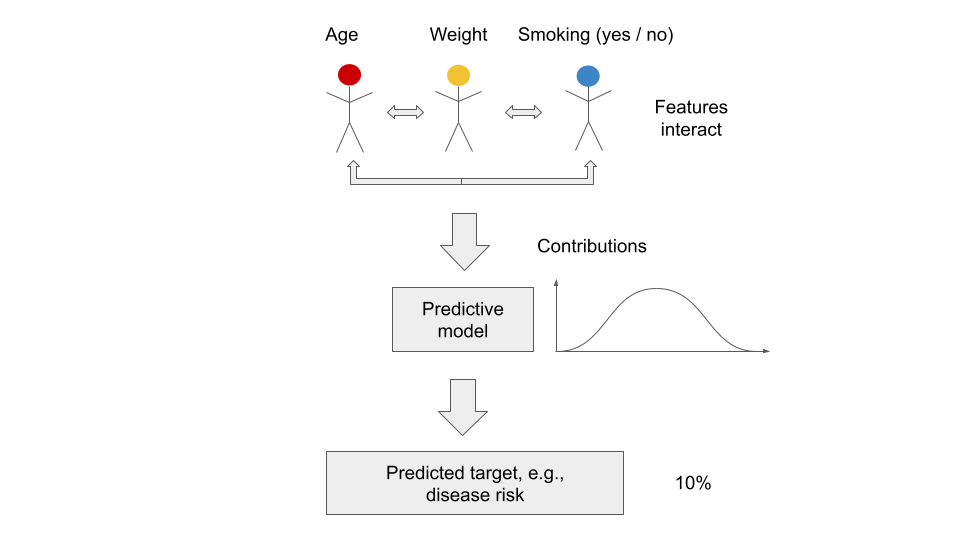
\includegraphics{figure/Shapley_6.png}
\end{figure}

\end{vbframe}

\begin{vbframe}{From Game Theory to Machine Learning}
\begin{itemize}
    \itemsep1em
    \item The features $x_j, j \in \pset$ represent the agents
    \item The game corresponds to the prediction $\fh(x_1, x_2, \ldots, x_p)$ for a single data observation $\xv$
    \item The features cooperate to produce a prediction
    \item The only issue is: How do we produce a prediction with a subset of features without changing the predictive model?
    \\ $\Rightarrow$ Partial dependence: $\fh_{S}(\xv_S) := \int_{X_C} \fh(\xv_S, X_C)d \P_{X_C}$
    \item  The value function / payout of coalition $S$ for observation $\xv$ is
    $$v(S) =  \fh_{S} (\xv_S) - \E_{\xv}(\fh(\xv)),$$ 
    where $\xv_S = \{x_j\}_{j \in S}$ and $\fh_S: \Xspace_S \mapsto \Yspace$ \\ $\leadsto$ the subtraction of $\E_{\xv}(\fh(\xv))$ is necessary so that $v$ is a value function with $v(\emptyset) = 0$
\end{itemize}
\end{vbframe}

% \begin{vbframe}{Shapley Values}
%   We can use Shapley values to explain individual predictions $\fh(\xv)$ of a machine learning model $\fh$:
% \begin{itemize}
%   \item Players $\hat{=}$ feature values of $i$-th observation $x_j, j \in \pset$.
%   \item Features cooperate to produce a prediction $\fh(x_1, x_2, \ldots, x_p)$.
%   \item The value function / payout of coalition $S$ for observation $\xv$ is
%     $$v(S) =  \fh_{S} (\xv_S) - \E_{\xv}(\fh(\xv)),$$ 
%     where $\xv_S = \{x_j\}_{j \in S}$ and $\fh_S: \Xspace_S \mapsto \Yspace$.
% \item The marginal prediction $\fh_S$ is defined as $\fh_{S}(\xv_S) := \int_{X_C} \fh(\xv_S, X_C)d \P_{X_C}$
% \item We have already seen the marginal prediction in action in the PDP.
% \item The subtraction of $\E_{\xv}(\fh(\xv))$ is necessary so that $v$ is a value function with $v(\emptyset) = 0$.
% \item By using the marginal prediction, we have defined what it means for features to be \enquote{missing} for the prediction: We remove it by integrating over its distribution.
% \end{itemize}
% \begin{center}
% \vspace{-0.3cm}
% 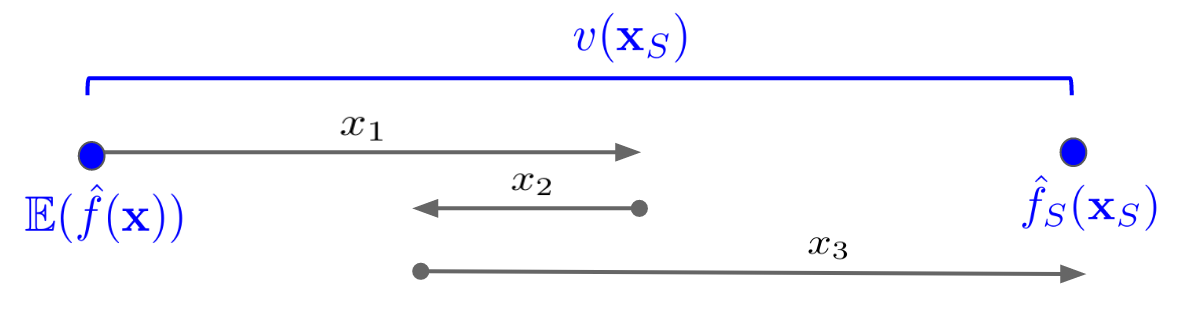
\includegraphics[width=0.6\textwidth]{figure_man/shapley_valuefct}
% \end{center}

% \begin{itemize}
%  \item Shapley values tell us what the payout of each feature is, i.e., how each feature contributes to the overall prediction of a specific observation.
%     \item The Shapley value is the average marginal contribution of a feature towards the prediction \textbf{across all possible feature coalitions}.
%     \item The sum of Shapley values over all features yields the difference between the average prediction of all data points (baseline) and the selected individual prediction.
%   \end{itemize}
% \end{vbframe}

\begin{vbframe}{Shapley Value - Definition \citebutton{Shapley (1953)}{https://doi.org/10.7249/P0295} \citebutton{Strumbelj et al. (2014)}{https://doi.org/10.1007/s10115-013-0679-x}}
  Using the order definition, the Shapley value for feature $j$ and a given data point $\xv$ can be computed as:

     $$ \phi_j  = \frac{1}{p!} \sum_{S \subseteq P\setminus \{j\}} \underbrace{\fh_{\Scupj}(\xv_{\Scupj}) - \fh_{S}(\xv_{S})}_{\text{marginal contribution of feature $j$}} $$
\begin{itemize}
    \item The term $\E_{\xv}(\fh(\xv))$ drops due to the subtraction of value functions
  \item Interpretation of Shapley value $\phi_j$ for feature $j$ and observation $\xv$:
  The feature value $x_j$ contributed $\phi_j$ towards the prediction $\fh(\xv)$ compared to the average prediction for the dataset.
   \item Note: Marginal contributions and Shapley values can be negative
\end{itemize}
\lz
%\tiny
%Shapley, Lloyd S. 1953. $"$A Value for N-Person Games.$"$\\
%\vspace{0.2cm}
%Strumbelj, Erik, Igor Kononenko, Erik Strumbelj, and Igor Kononenko. 2014. $"$Explaining prediction models and individual predictions with feature contributions.$"$

\end{vbframe}



\begin{vbframe}{Revisited: Axioms for Fair Attributions}
  We take the general axioms for Shapley Values and apply it to predictions:
  \vspace{0.25cm}
  \begin{itemize}
  \itemsep1em
    \item \textbf{Efficiency}: Feature contributions add up to the (centered) prediction. That means, unlike, e.g., LIME, we get a dense attribution, and not a sparse one.
      $\sum\nolimits_{j=1}^p\phi_j=\fh(\xv)-\E_{\xv}(\fh(X))$
    \item \textbf{Symmetry}: Two features that contribute the same to the prediction get the same payout $\leadsto$ interaction effects between two features are fairly divided. \\
      $\fh_{S\cup\{j\}}(\xv_{\Scupj}) = \fh_{\Scupk}(\xv_{\Scupk})$ for all $S \subseteq P\setminus\{j,k\}$ then $\phi_j=\phi_k$
    \item \textbf{Dummy / Null Player}: Shapley value of a feature that does not influence the prediction is zero $\leadsto$ if a feature was not selected by the model (e.g., tree or LASSO) the Shapley value is zero  \\
      $\fh_{\Scupj}(\xv_{\Scupj})=\fhS(\xv_S)$ for all $S \subseteq P$ then $\phi_j=0$
    \item \textbf{Additivity}:  For a prediction with combined payouts, the
      payout is the sum of payouts: $\phi_j(v_1) + \phi_j(v_2)$ $\leadsto$ Shapley values for model ensembles can be combined
  \end{itemize}
\end{vbframe}



\begin{vbframe}{Estimation: A practical problem}
  \begin{itemize}
  \itemsep1em
      \item Feature space is often high-dimensional
      \item High-dimensionality is problematic for the (exact) Shapley value computation: For only 10 features, there are already $10! \approx 3.6$ million possible orders of features
      \item We have a similar problem with the estimation of the marginal prediction: Averaging over the entire dataset for each (sampled) coalition would be very expensive
      \item The solution to both problems is sampling: We calculate the Shapley value over $M$ samples -- for each sample, we sample one order of features and one data point to replace missing features
      \item $M$ is a tradeoff between accuracy of the Shapley value and computational costs -- the higher $M$, the closer we get to the true Shapley values, but the more costly the computation becomes
  \end{itemize}
\end{vbframe}

\newcommand{\xk}{\mathbf{x}^{(k)}}

\begin{vbframe}{Estimation Algorithm \citebutton{Strumbelj et al. (2014)}{https://doi.org/10.1007/s10115-013-0679-x}}
Estimation of $\phi_j$ for model $\fh$, observation $\xv$, and sample size $M$:
\vspace{0.25cm}
  \begin{enumerate}
      \item For m in 1 to M, \textbf{do}:
      \begin{enumerate}
        \item Select random permutation $\pi \in \Pi$.
        \item Select random data point $\xv^{(k)} \in X$.
        \item Order $\xv$ according to $\pi$: $\xv_{\pi} = (x_{\pi(1)}, \ldots, x_{\pi(j)}, \ldots, x_{\pi(p)})$.
        \item Order $\xk$ according to $\pi$: $\xk_{\pi} = (x^{(k)}_{\pi(1)}, \ldots, x^{(k)}_{\pi(j)}, \ldots, x^{(k)}_{\pi(p)})$.
        \item Construct two observations:
          \begin{itemize}
          \setlength\itemsep{.5em}
            \item $\xv_{+j} = (x_{\pi(1)}, \ldots, x_{\pi(j - 1)}, x_{\pi(j)}, x^{(k)}_{\pi(j + 1)}, \ldots, x^{(k)}_{\pi(p)}) $
            \item $\xv_{-j} = (x_{\pi(1)}, \ldots, x_{\pi(j - 1)}, x^{(k)}_{\pi(j)}, x^{(k)}_{\pi(j + 1)}, \ldots, x^{(k)}_{\pi(p)}) $
          \end{itemize}
        \item Compute difference $\phi_j^m = \fh(\xv_{+j}) - \fh(\xv_{-j})$.
      \end{enumerate}
    \item Compute Shapley value $\phi_j = \frac{1}{M}\sum_{m=1}^M \phi_j^m$.
  \end{enumerate}

  Each $\phi_j^m$ is a sample from the marginal contribution for a sampled coalition.

   % \vspace{0.25cm}
    %\tiny{Strumbelj, Erik, Igor Kononenko, Erik Strumbelj, and Igor Kononenko. 2014. $"$Explaining prediction models and individual predictions with feature contributions.$"$}

\end{vbframe}

\begin{vbframe}{Excursus: SHapley value computation}

\begin{exampleblock}{Definition}
\[
\tikzmark{phi}\phi_{\tikzmark{j}j}(\tikzmark{v}\fh, \tikzmark{x}\xv)=\frac{1}{M}\tikzmark{M}\sum_{m=1}^M \left[\fh_{S_m \tikzmark{SJ}\cup j}\left(\xv_{S_m \tikzmark{SJ}\cup j} \right)-\fh_{\tikzmark{S}S_m}\left(\xv_{\tikzmark{S}S_m}\right)\right]
\]
\begin{tikzpicture}[
  remember picture,
  overlay,
  expl/.style={draw=blue,fill=white,rounded corners,text width=3cm},
  arrow/.style={blue,ultra thick,->,>=latex}
]
%%%% Explain Formula I
\draw<2-3> [draw=white, fill=white, opacity=0.6]
       (5.8,0) -- (11,0) -- (11,2) -- (5.8,2) --cycle;
\node<2>[expl] 
  (phiex) 
  at (6,2cm)
  {$\phi$: The Shapley value};
\node<2>[expl] 
  (jex) 
  at (2,0cm)
  {for feature $j$};
\node<3>[expl] 
  (vex) 
  at (5,-0.7cm)
  {$\fh$: pred. function};
\node<3>[expl] 
  (xex) 
  at (6,2cm)
  {$x$: Input data (a single observation)};
\draw<2>[arrow]
  (phiex.south) to[out=270,in=90] ([xshift= 1ex, yshift=1.5ex]{pic cs:phi});  
\draw<2>[arrow]
  (jex.north) to[out=90,in=270] ([yshift=-0.5ex]{pic cs:j});  
\draw<3>[arrow]
  (vex.east) to[out=0,in=270] ([xshift= 1ex, yshift=-0.5ex]{pic cs:v});  
\draw<3>[arrow]
  (xex.west) to[out=180,in=135] ([xshift= 1ex, yshift=1ex]{pic cs:x}); 
  
 %%%% Explain Formula II
\draw<4-5> [draw=white, fill=white, opacity=0.6]
       (4,0) -- (6.8,0) -- (6.8,2) -- (4,2) --cycle;
\node<4>[expl] 
  (Sex) 
  at (10,2cm)
  {$x_{S_m}$: A subset of $x_S$};
\node<5>[expl] 
  (Sex) 
  at (13,1cm)
  {$\fh_{S_m}(x_{S_m})$: The contribution of $x_{S_m}$ to the prediction};
 \node<4>[expl] 
  (SJex) 
  at (10,-0.8cm)
  {$x_{S_m \cup j}$: The same subset $x_{S_m}$ but including feature $j$};
  \draw<4>[arrow]
  (Sex.south) to[out=270,in=90] ([xshift= 1ex, yshift=1.5ex]{pic cs:S});
 \draw<5>[arrow]
  (Sex.north) to[out=90,in=90] ([xshift= 1ex, yshift=1.5ex]{pic cs:S});
  \draw<4>[arrow]
  (SJex.north) to[out=90,in=270] ([yshift=-0.5ex]{pic cs:SJ}); 
  \draw<5> [decorate,decoration={brace, amplitude=5pt,mirror,raise=4ex}]  (7.4,1.1) --  (10.5,1.1)
  node[midway,yshift=-3.5em]{$:= \Delta(j, S_m)$};
  %%%% Explain Formula III
  \draw<6> [draw=white, fill=white, opacity=0.6]
       (4,0) -- (5.7,0) -- (5.7, 2) -- (4,2) --cycle;
  \draw<6> [draw=white, fill=white, opacity=0.6]
        (6.8,0) -- (12,0) -- (12,2) -- (6.8,2) --cycle;
  \node<6>[expl] 
  (Mex) 
  at (12,2cm)
  {$\frac{1}{M}\sum$: Average the contribution of feature $j$};
  \draw<6>[arrow]
  (Mex.west) to[out=180,in=90] ([xshift= 0.5ex, yshift=4ex]{pic cs:M}); 
\end{tikzpicture}
\end{exampleblock}
\vspace{0.5cm}
\begin{itemize}
    \begin{onlyenv}<2>
    \item The Shapley value assigns a value to each feature $j$ according to the marginal contribution of each player in all possible coalitions $S$.
    \end{onlyenv}
    %\begin{onlyenv}<3>
    %\item A value function $v(S): 2^{|P|}\mapsto \R$ describes the payout (or gain) achieved by any coalition $\forall S \subseteq P$. The value of the empty coalition must be zero: $v(\emptyset) = 0$.
    %\item The payout of coalition $S$ for observation $\xv$ is 
    %$$v(\xv_S) =  \fh_{S} (\xv_S) - \E (\fh(\xv))$$ 
    %i.e., the difference of the marginal prediction of $\xv_S$ and the average prediction.
    %\end{onlyenv}
    %\begin{onlyenv}<4>
    %\item Example observation from bike sharing data
    %\end{onlyenv}
    % Part II
    %\begin{onlyenv}<5>
    %\item $S_m$ is a randomly selected set of features: $S_m \subseteq P \setminus j$ where $P$ denotes the quantity of all features in $X$
    %\item Let $x_{S_m}$ be a random chosen subset of features in $x_S$ that is hold fix
    %\end{onlyenv}
     %   \begin{onlyenv}<6>
    %\item Let $S_{\lnot m}$ denote the subset of $P$ that is not in $S_m$.
    %\item Draw the values of all other features $x_{S_{\lnot m}}$ randomly from the set of available values of the regarding feature to calculate $v(x_{S_m})$
    %\end{onlyenv}
    \begin{onlyenv}<5>
     \item $\Delta(j, S_m) = \fh_{S \cup j}(x_{S \cup j}) - \fh_S(x_{S})$ is the marginal contribution of player $j$ to coalition $S$
    \item In this subset $S_m$ the variable \textit{year} contributes +17 bike rentals compared to the expected prediction conditioned on features in $S_m$ (and all other features are assumed to be absent)
    \end{onlyenv}
    \begin{onlyenv}<6>
    \item Average the marginal contribution of feature $j$ towards the prediction
    across all randomly drawn feature coalitions $S_1, \ldots , S_M$.
    \item The resulting Shapley value $\phi_j$ tells us what the payout of feature $j$ is, i.e., how the feature \textit{year} contributes to the overall prediction in bicycle counts of a specific observation $\xv$
    \end{onlyenv}
\end{itemize}
\vspace*{\fill}
\begin{center}
%\includegraphics<3>[width=0.5\textwidth]{figure_man/shapley_valuefct}
% Link https://docs.google.com/presentation/d/14FZZ4zk7IBZv6XnQA0wDVfCDhmjzf4np5uVj7KrIxXg/edit#slide=id.p
%\includegraphics<4>[page=1, width=1\textwidth]{figure_man/data_shapley}
%\includegraphics<5>[page=2, width=1\textwidth]{figure_man/data_shapley}
%\includegraphics<6>[page=3, width=1\textwidth]{figure_man/data_shapley}
%\includegraphics<7>[page=4, width=1\textwidth]{figure_man/data_shapley}
\includegraphics<5>[page=5, width=1\textwidth]{figure_man/data_shapley}
\includegraphics<6>[page=6, width=1\textwidth]{figure_man/data_shapley}
\end{center}

\end{vbframe}

\begin{vbframe}{Additional Estimation Trick}


  The Shapley value can be estimated more efficiently when certain coalitions are always included in the computation, instead of random sampling:
  \vspace{0.25cm}
  \begin{itemize}
  \itemsep1em
    \item The coalitions with $S = \emptyset$ (i.e., $|S| = 0$) and $S = \{1, \ldots, p\} \setminus j$ have the highest weights in the Shapley value computation $\leadsto$ including them makes Shapley value more stable with fewer samples %Sample weights have to be adapted for the sampled coalitions afterwards.
    \item Intuition: Adding a feature to the empty coalition gives information about the \textit{pure} first order effect of the feature, which is the effect without any interactions 
    \item Adding the feature value to the complete set of feature values gives us the information about the total effect of a feature, which is the sum of the main effect and all interaction effects with other features
    \item For coalition $S = \emptyset$, there are $0! (|P| - 0 - 1)! = 1 \cdot (|P| - 1)! = (p - 1)!$ orders, which is the same for $S = P \setminus \{j\}$: $|P \setminus \{j\}|! (|P| - |P \setminus \{j\}| - 1)! = (p - 1)! (p - (p-1) - 1)! = (p-1)!$
\end{itemize}
 \end{vbframe}

\begin{vbframe}{Additional Estimation Trick}
An example with $p = 5$ features:
\vspace{0.25cm}
    \begin{itemize}
    \itemsep1em
        \item There are $5! = 120$ orders in total
        \item In $(5 - 1)! = 24$ orders, we added feature value $x_j$ to the empty set
        \item In 24 orders, we added the feature value to the otherwise full feature set
        \item That means with just two sets, we can already get $\frac{48}{120} = 0.4$ of the contributions to the Shapley value
        \item Similarly, we could proceed with all coalitions of $\{S: |S| = 1\}$ and $\{S: |S| = p - 1\}$
        \item When some coalitions are added \enquote{manually}, and the rest are sampled, we have to adapt the weights: Let $w$ be the weight of the \enquote{manually} sampled coalitions, $\hat{\phi}_{j,fixed}$ the part of the Shapley value with only the manual contributions and $\hat{\phi}_{j,sample}$ the Shapley value with the sampled coalitions, then the Shapley value is: $w \cdot \hat{\phi}_{j,fixed} + (1 - w) \hat{\phi}_{j,sample}$
  \end{itemize}
\end{vbframe}

\begin{vbframe}{Additional Estimation Trick}
      \begin{center}
        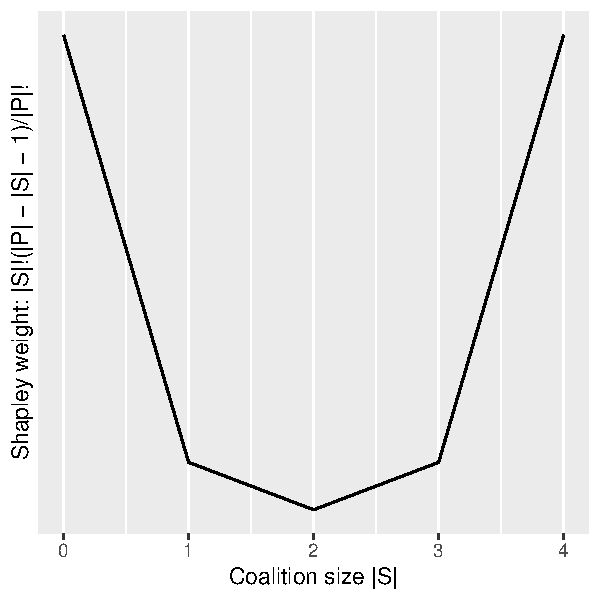
\includegraphics[width=0.5\textwidth]{figure/shapley-weights}
      \end{center}
\end{vbframe}

\begin{vbframe}{Bike Sharing Dataset}

\begin{center}
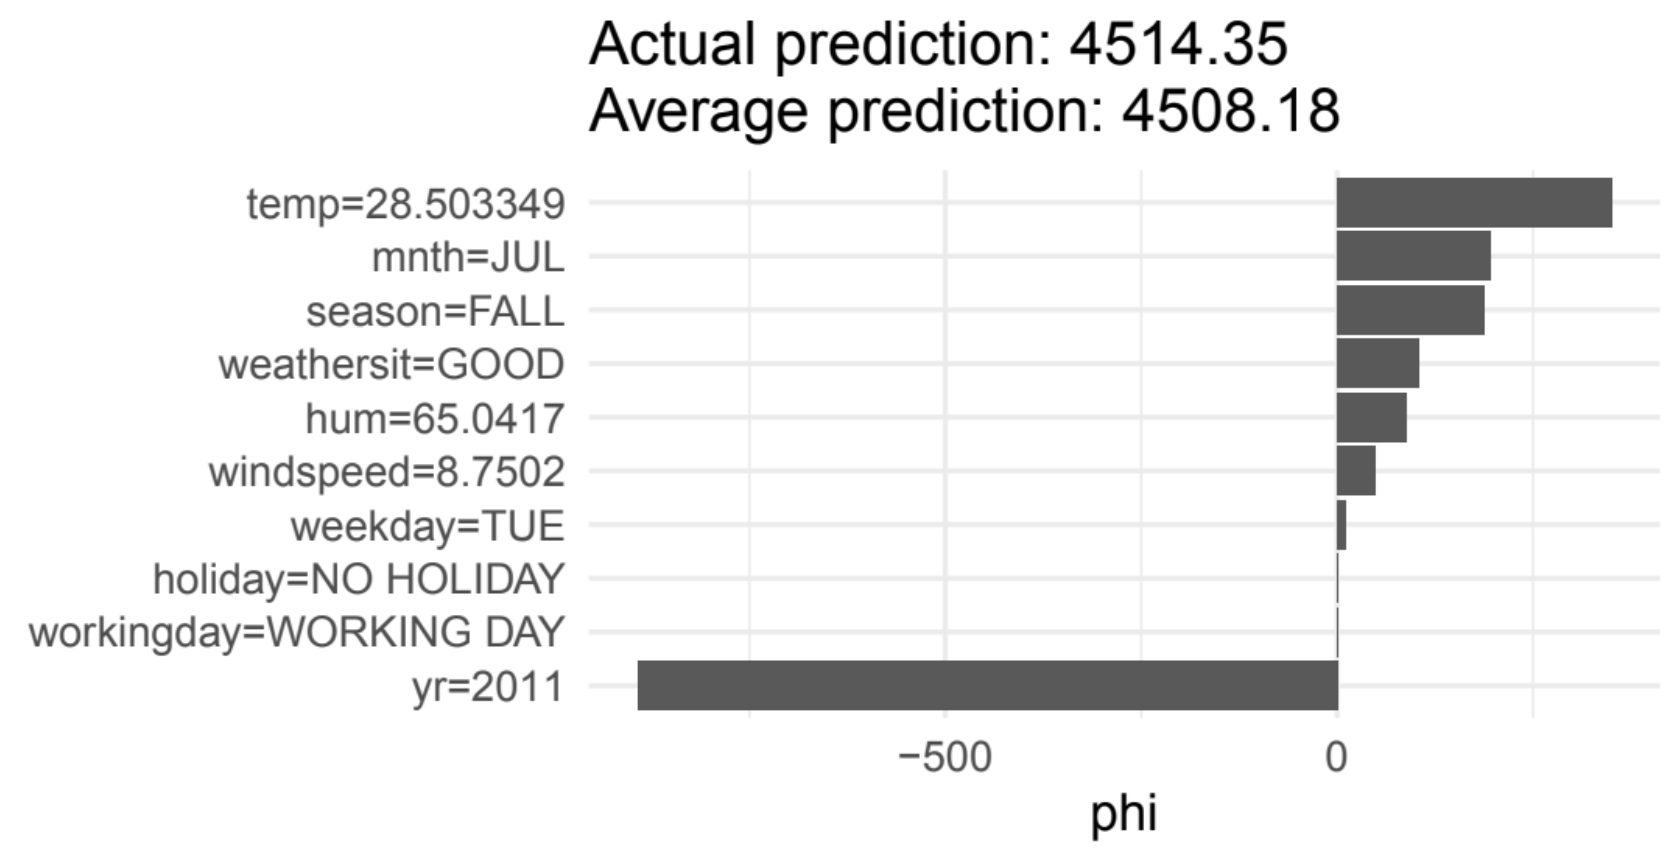
\includegraphics[width=0.6\textwidth]{figure_man/bike-sharing03.png}
\end{center}

\begin{itemize}
    \item The plot shows the Shapley values for observation 200 in the Bike Sharing data
    \item The difference between the model prediction of this observation and the average prediction of the data is fairly distributed among the features (i.e., 4514 - 4508)
    \item Feature value temp = 28.5 has the most positive effect, with a contribution (increase of prediction) of + 350
\end{itemize}
\end{vbframe}

% \begin{vbframe}{Versions of the Shapley Value}

%   \begin{itemize}
%   \item KernelSHAP formulates the Shapley value solution as a regression problem using a specific kernel function. The authors show paralles to LIME and Deeplift.
%   \item TreeSHAP is a fast Shapley value computation method for tree-based models such as gradient boosted trees.
%  \end{itemize}
%     \tiny{Lundberg, Scott M., and Su-In Lee. "A Unified Approach to Interpreting Model Predictions." Advances in Neural Information Processing Systems 30 (2017): 4765-4774.}
%     \tiny{Lundberg, Scott M., Gabriel G. Erion, and Su-In Lee. "Consistent individualized feature attribution for tree ensembles." arXiv preprint arXiv:1802.03888 (2018).}
% \end{vbframe}

\begin{vbframe}{ADVANTAGES AND DISADVANTAGES}
	\textbf{Advantages:}
	\begin{itemize}
	 \item \textbf{Solid theoretical foundation} in game theory
        \item Prediction is \textbf{fairly distributed} among the feature values
        \item \textbf{Contrastive explanations} that compare the prediction with the average prediction
	\end{itemize}
\vspace{0.25cm}
	\textbf{Disadvantages:}
	\begin{itemize}
		\item 	Without sampling, Shapley values need a lot of computing time to
		inspect all possible coalitions
		\item The Shapley value of a feature value can be easily misinterpreted:
		It is not the difference of the predicted value after removing the
		feature from the model training; it is the contribution of a feature
		value to the difference between the actual prediction and the mean
		prediction, given the current set of features
		\item Like many other IML methods, Shapley values suffer from the
		inclusion of unrealistic data observations when features are
		correlated
	\end{itemize}



\end{vbframe}

\endlecture
\end{document}
